\documentclass{beamer}

\usepackage[absolute,overlay]{textpos}

\begin{document}
  \begin{frame}[t]\frametitle{Buzzwords}
    \begin{itemize}
      \item drawing program
      \item non destructive
      \item procedural
      \item object oriented
      \item structured
      \item programmable
      \item wysiwym
      \item wysiwyg
      \item 2D + time
    \end{itemize}
  \end{frame}

  \begin{frame}[t]\frametitle{Related software}
    \begin{itemize}
      \item Inkscape: 
        \begin{itemize}
          \item similar use case, similar target audience
          \item not as well structured
          \item \textbf{focuses on the result rather on the way to it}
        \end{itemize}
      \item \LaTeX+TikZ, python+matplotlib, \dots
        \begin{itemize}
          \item power of programming language/\LaTeX
          \item horribly to use (I like it)
          \item lack of immediate visual feedback
          \item wysiwym, variables, dependencies, \dots
        \end{itemize}
      \item Cinema 4D:
        \begin{itemize}
          \item 3D modelling/animation/rendering application
          \item inspiring concepts and ui
        \end{itemize}
    \end{itemize}
  \end{frame}

  \begin{frame}[t]\frametitle{Motivation}
    \begin{textblock*}{5cm}(7.6cm,0.5cm) % {block width} (coords)
      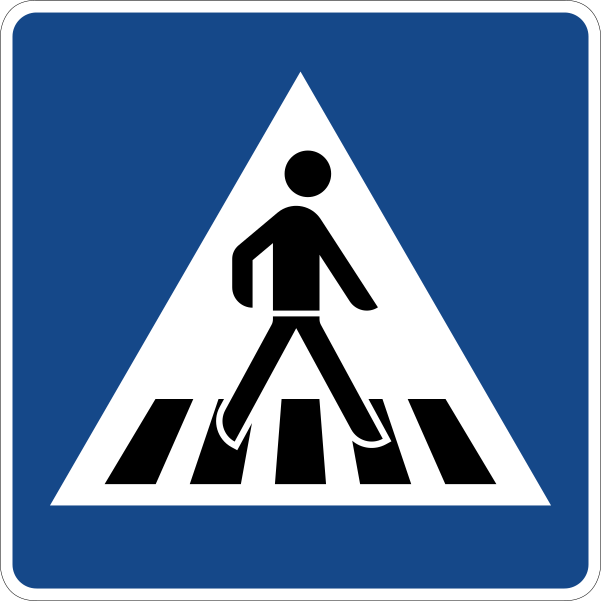
\includegraphics[width=\textwidth]{media/601px-Zeichen_350-20_-_Fußgängerüberweg_(Linksaufstellung)_einseitig,_StVO_1992.png}
    \end{textblock*}
    \begin{itemize}
        \item task: draw a \\pedestrian crossing sign
        \item easy-peasy with Inkscape
        \item but then: increase the margin
        \begin{itemize}
           \item fiddling to align it
        \end{itemize}
        \item change the color of the stripes
        \begin{itemize}
          \item must select each one separately
        \end{itemize}
        \item imagine more complicated \\
        drawings with inner dependencies
        \begin{itemize}
          \item A has same color as B
          \item A and B have common center
          \item A and B have common top-left
          \item $\text{A.x} = -\text{B.x}$
          \item $\text{A.x}\cdot\cosh({\text{A.color.r}}) = \sqrt{\text{B.y} - \text{B.color.b}}$
        \end{itemize}
      \end{itemize}  
  \end{frame}

  \begin{frame}[t]\frametitle{Analogy: Programming}
    \begin{itemize}
      \item extract repeating code parts: functions
      \begin{itemize}
        \item don't repeat yourself!
      \end{itemize}
      \item abstract from values: variables, constants
      \begin{itemize}
        \item reduce redundancy, make changes easily applicable
      \end{itemize}
      \item encapsulation
      \begin{itemize}
        \item reveal only what is relevant, hide implementation detail
      \end{itemize}
    \end{itemize} 
  \end{frame}

  \begin{frame}[t]\frametitle{Concept}
    \begin{itemize}
      \item central ``thing'': \textbf{Object}
      \begin{itemize}
        \item coordinate system
        \item propertie
        \begin{itemize}
          \item name
          \item position, rotation (cf. coordinate system)
          \item radius/interpolation/\dots
        \end{itemize}
        \item exactly one parent object (except root)
        \item zero or more child objects
        \item maybe geometry
        \begin{itemize}
          \item \empty{circle}, \empty{path}, \empty{empty}, \dots
        \end{itemize}
      \end{itemize}
    \item ui
      \begin{itemize}
        \item object-manager: modify object hierarchy
        \item property-manager: modify object proprties
        \item viewport: interactive visual feedback
      \end{itemize}
    \end{itemize}
  \end{frame}

  \begin{frame}[t]\frametitle{Concept}
    \begin{itemize}
      \item how to realize ``functions''?
      \item macros!
      \item but: super-easy to use: \\users don't realize they've just recorded/used a macro
      \item idea: freeze an object with a single click:
        \begin{itemize}
          \item makes children invisible, unselectable in object-manager
          \item object can then be copied or instanciated
          \item instances can have different property values and hence can have different appearance
          \item encapsulated the implementation detail of the frozen object behind the simple interface of (user-defined) properties.
          \item analogy: calling the same function with different arguments
        \end{itemize}
      \item can be ``unfreezed'' at any point 
      \item project (file) specific template library
      \item standard library with advanced objects
    \end{itemize}
  \end{frame}

  \begin{frame}[t]\frametitle{Concept}
    \begin{itemize}
      \item Scripting
      \begin{itemize}
        \item every property shall be readable and writable with a scripting language
        \item like blender+python
        \item scripts can be tied to an object
        \item scripts can silently duplicate objects (not visible in object-manager)
        \item simple utilization: freeze \texttt{empty}+script $\rightarrow$ instance-object
        \item advanced utilization: cloner-object with sophisticated options
        \item provided by standard libary
      \end{itemize}
    \end{itemize}
  \end{frame}

  \begin{frame}[t]\frametitle{Properties}
    \begin{itemize}
      \item name $\rightarrow$ value: type
      \item types: string, float, integer, option, bool, object, reference, color, curve, gradient, \dots
      \item depending on type, additional info is stored:
      \begin{itemize}
        \item float: min, max, step
        \item option: options (list of strings)
        \item \dots
      \end{itemize}
      \item editing multiple objects
      \begin{itemize}
        \item select two or more objects
        \item property manager shows intersection of properties
        \item all objects have same value: no problem
        \item at least two different values: show hint
        \item properties of all selected objects can be set at once
        \item value-aware editing: \texttt{+1}, \texttt{3*x+1}, \texttt{A.x + B.y}
      \end{itemize}
      \item categories: \texttt{General/Name}, \texttt{Circle/Radius}
    \end{itemize}
  \end{frame}

  \begin{frame}[t]\frametitle{Tags}
    \begin{itemize}
      \item add additional functionality to an object
      \item e.g. script-tag
      \begin{itemize}
        \item most versatile, but not intuitive to use
        \item all other tags are just predefined script tags
      \end{itemize}
      \item constrain-tag: tie object property to some other property
    \end{itemize}
  \end{frame}

  \begin{frame}[t]\frametitle{Style}
    \begin{itemize}
      \item brush: pattern, color
      \item pen: line style, line width, color
    \end{itemize}
  \end{frame}

  \begin{frame}[t]\frametitle{Animation}
    \begin{itemize}
      \item global time line
      \item provisional: time-dependent scripts
      \item later: key frame interpolation
    \end{itemize}
  \end{frame}

  \begin{frame}[t]\frametitle{Open questions}
    \begin{itemize}
      \item Z-order?
      \item file format: json/svg/binary/\dots
      \item scripting language: python3?
      \item backend (library): C++ ?
      \item frontend (GUI): C++/Qt, C/gtk, \dots ?
    \end{itemize}
  \end{frame}

\end{document}